%; whizzy paragraph
%; whizzy-paragraph "^\\\\dancersection"
% -initex iniptex -latex platex -format platex -bibtex jbibtex -fmt fmt
% 以上 whizzytex を使用する場合の設定。

%     Tokyo Debian Meeting resources
%     Kansai Debian Meeting resources
%     Copyright (C) 2008 Junichi Uekawa
%     Copyright (C) 2008 Nobuhiro Iwamatsu

%     This program is free software; you can redistribute it and/or modify
%     it under the terms of the GNU General Public License as published by
%     the Free Software Foundation; either version 2 of the License, or
%     (at your option) any later version.

%     This program is distributed in the hope that it will be useful,
%     but WITHOUT ANY WARRANTY; without even the implied warranty of
%     MERCHANTABILITY or FITNESS FOR A PARTICULAR PURPOSE.  See the
%     GNU General Public License for more details.

%     You should have received a copy of the GNU General Public License
%     along with this program; if not, write to the Free Software
%     Foundation, Inc., 51 Franklin St, Fifth Floor, Boston, MA  02110-1301 USA

%   Pdf作成手順
% dvipdfmx debianmeetingresume2011-fuyu.dvi
%  preview (shell-command (concat "evince " (replace-regexp-in-string "tex$" "pdf"(buffer-file-name)) "&"))
% 画像ファイルを処理するためにはebbを利用してboundingboxを作成。
%(shell-command "cd image2012-fuyu; ebb *.png")


% progress memo:
% 2018/6 kansai-2018/11がマージ対象
% イベント等でない場合は理由を書くこと。
% 必要な変更点は FIXME で記録しています。

%%ここからヘッダ開始。

\documentclass[mingoth,a4paper]{jsarticle}
\usepackage{monthlyreport}
\usepackage[dvips]{xy} % for advi workaround. Bug #452044
\usepackage{ulem}
\usepackage{wrapfig}

% ページ調整のため部分的に2段組に
\usepackage{multicol}

\begin{document}

\begin{titlepage}
\thispagestyle{empty}

\hspace*{-2.5cm}
\includegraphics{image2012-natsu/gudeb.eps}\\
\\
\\
\rotatebox{10}{\fontsize{32}{32} {\gt 東京エリア/関西Debian勉強会}}

%\vspace*{-1.5cm}
\hspace*{11cm}
\includegraphics[height=6cm]{image200502/openlogo-nd.eps}\\
\vspace*{0.1cm}
\hfill あんどきゅめんてっど でびあん 2018年冬号 2018年12月30日 初版発行
\end{titlepage}

\newpage
\thispagestyle{empty}\mbox{}
\newpage

% section の代わりの環境 -- 改訂する。
\renewcommand{\dancersection}[2]{%
\newpage
あんどきゅめんてっど でびあん 2017年冬号
%
% top line
\vspace{0.1mm}\\
{\color{dancerlightblue}\rule{\hsize}{2mm}}

%
% middle text
%
\begin{minipage}[t]{0.6\hsize}
\color{dancerdarkblue}
\vspace{1cm}
\section{#1}
\hfill{}#2\\
\end{minipage}
\begin{minipage}[t]{0.4\hsize}
\vspace{-2cm}
\hfill{}
\includegraphics[height=8cm]{image200502/openlogo-nd.eps}\\
\vspace{-5cm}
\end{minipage}
%
%
{\color{dancerdarkblue}\rule{0.74\hsize}{2mm}}
%
\vspace{2cm}
}

\setcounter{page}{1}
\begin{minipage}[]{0.2\hsize}
 \definecolor{titleback}{gray}{0.9}
 \colorbox{dancerlightblue}{\rotatebox{90}{\fontsize{80}{80}
{\gt \color{dancerdarkblue}デビアン勉強会} }}
\end{minipage}
\begin{minipage}[]{0.8\hsize}
\hrule
\vspace{1mm}
\hrule
\setcounter{tocdepth}{1}
{\small
 \tableofcontents}
\vspace{1mm}
\hrule
\vspace{3cm}

\end{minipage}

% FIXME: 本文を追加すること。
%-------------------------------------------------------------------------------
\dancersection{Introduction}{DebianJP}
%-------------------------------------------------------------------------------

\subsection{東京エリアDebian勉強会}

 Debian勉強会へようこそ。これからDebianの世界にあしを踏み入れると
 いう方も、すでにどっぷりとつかっているという方も、月に一回Debianについ
 て語りませんか?

 Debian勉強会の目的は下記です。

\begin{itemize}
 \item \underline{Debian Developer} (開発者)の育成。
 \item 日本語での ``\underline{開発に関する情報}'' を整理してまとめ、アップデートする。
 \item \underline{場}の提供。
 \begin{itemize}
  \item 普段ばらばらな場所にいる人々が face-to-face で出会える場を提供
    する。
  \item Debian のためになることを語る場を提供する。
  \item Debianについて語る場を提供する。
 \end{itemize}
\end{itemize}

 Debianの勉強会ということで究極的には参加者全員がDebian Packageをがりがり
 と作るスーパーハッカーになった姿を妄想しています。情報の共有・活用を通し
 て Debianの今後の能動的な展開への土台として、 ``場'' としての空間を提供す
 るのが目的です。

\subsection{関西 Debian 勉強会}

 関西 Debian 勉強会はDebian GNU/Linux のさまざ
 まなトピック(新しいパッケージ、Debian 特有の機能の仕組、Debian 界隈で起
 こった出来事、などなど)について話し合う会です。

 目的として次の三つを考えています。
 \begin{itemize}
  \item MLや掲示板ではなく、直接顔を合わせる事での情報交換の促進
  \item 定期的に集まれる場所
  \item 資料の作成
 \end{itemize}

 それでは、楽しい一時をお楽しみ下さい。
 
%収録予定
%debianmeetingresume201809.tex: \dancersection{Rethinking of debian/watch rule}{Kentaro Hayashi (@kenhys)}
%debianmeetingresume201808.tex: \dancersection{DebConf18参加報告}{DebConf18に参加した方々} https://tokyodebian-team.pages.debian.net/2018-08_tokyodebian_debconf18_bof.txt
%debianmeetingresume201811.tex: \dancersection{debianにおけるnginxの設定例}{杉本 典充}
%以下印刷用に要再編集
%debianmeetingresume201807-meetup-sapporo-presentation-sugimoto.tex    \title{Debian / Ubuntu ユーザーミートアップ in 札幌 2018.07 \\ \\Debianで自宅にリモート接続 / OpenVPN編} 杉本 典充
%debianmeetingresume201807-meetup-sapporo-presentation-yyoshino.tex    \title{Debian で Atom、\\Debian で Visual Studio Code} 吉野 与志仁
%下記いずれか or mix
%debianmeetingresume201807-osc2018do-presentation.tex    Debian Updates \& Random Topics 佐々木
%debianmeetingresume201810-osc2018fall-presentation.tex Debian Updates & debconf 杉本


%-------------------------------------------------------------------------------
%debianmeetingresume201807-meetup-sapporo-presentation-sugimoto.tex    \title{Debian / Ubuntu ユーザーミートアップ in 札幌 2018.07 \\ \\Debianで自宅にリモート接続 / OpenVPN編} 杉本 典充
\dancersection{Debianで自宅にリモート接続 / OpenVPN編}{杉本 典充}
%-------------------------------------------------------------------------------

\subsection{アジェンダ}

\begin{itemize}
\item 自己紹介
\item VPNについて
\item OpenVPNの紹介
\item OpenVPNの設定(サーバ、クライアント)
\item おわりに
\item 参考資料
\end{itemize}


\subsection{自己紹介}

\begin{itemize}
\item Norimitsu Sugimoto (杉本 典充)
\item dictoss@live.jp
\item Twitter: @dictoss
\item 大学生のときからDebianを使っています
\item 仕事はソフトウェア開発者をやってます
\end{itemize}


\subsection{VPNについて}

\begin{itemize}
\item IPsec系
  \begin{itemize}
  \item L2TP/IPsec
  \end{itemize}
\item SSL-VPN系
  \begin{itemize}
  \item SSTP
  \item SoftEther
  \item OpenVPN
  \end{itemize}
\item 利用を推奨しない過去の技術
  \begin{itemize}
  \item PPTP(セキュリティ強度が低く、突破済み)
  \end{itemize}
\end{itemize}

\newpage

\subsection{OpenVPNの紹介}

\begin{itemize}
\item SSL-VPNを使ったVPN接続を行うソフトウェア
\item \url{https://openvpn.net/}
\item ライセンスはGPLv2
\item TLS 1.0〜TLS 1.2による暗号通信をサポート
\item サーバ側の機能とクライアント側の機能の両方をもつ
\item デフォルトのポート番号は1194/UDPで、TCPも利用可能
\end{itemize}

\subsection{DebianにおけるOpenVPN}

\begin{itemize}
\item Debian 8
  \begin{itemize}
  \item openvpn-2.3.4、openvpn-2.4.0(jessie-backports)
  \end{itemize} 
\item Debian 9
  \begin{itemize}
  \item openvpn-2.4.0、openvpn-2.4.4(stretch-backports)
  \end{itemize}
\item openvpnの2.3系と2.4系の違い
  \begin{itemize}
  \item 2.3.3からTLS 1.2が利用可能。ただし使える暗号はTLS 1.0由来のものに限られる(AES-CBC、RSA、DHE)
  \item 2.4からAES-GCMや、ECDHE、ECDSAなどTLS-1.2で利用可能な高度な暗号をサポート
  \item サーバとクライアントで2.3系と2.4系が混在する場合、古いバージョンがサポートする設定に合わせる必要がある
  \end{itemize}
\end{itemize}


\subsection{OpenVPNの設定の解説}

\subsubsection{OpenVPNの設定(サーバ)}

\begin{itemize}
\item "apt-get install openvpn" でインストール
\item 証明書や鍵の生成(easy-rsa 2)\footnote{\url{https://openvpn.net/index.php/open-source/documentation/miscellaneous/77-rsa-key-management.html}}
\item サーバ側の設定のサンプル\footnote{\url{https://github.com/OpenVPN/openvpn/blob/master/sample/sample-config-files/server.conf}}
\item 設定ファイルは''/etc/openvpn/*.conf''を使用し、複数のVPN設定を同時実行するマルチインスタンスが可能
  \begin{itemize}
  \item 例)443/TCPと1194/UDPの両方をlistenする
  \end{itemize}
\end{itemize}

\subsubsection{OpenVPNの設定(サーバ側を一部抜粋)}

\begin{commandline}
tls-server
tls-version-min 1.2
port 443
proto tcp
dev tun0
persist-key
persist-tun
push ``dhcp-option DNS 192.168.2.1''
push ``route 192.168.2.0 255.255.255.0''
client-to-client
client-config-dir /etc/openvpn/ccd
tls-auth /etc/openvpn/easy-rsa/2.0/keys/ta.key 0
  (snip)  
\end{commandline}

\newpage

\subsubsection{OpenVPNの設定(クライアント)}

\begin{itemize}
\item "apt-get install openvpn" でインストール
\item クライアント側の設定のサンプル\footnote{\url{https://github.com/OpenVPN/openvpn/blob/master/sample/sample-config-files/client.conf}}
\item 設定ファイルは、"/etc/openvpn/client.conf"とすること
\item systemctl start openvpn で起動
\end{itemize}


\subsubsection{OpenVPNの設定(クライアント側を一部抜粋)}

\begin{commandline}
client
tls-client
tls-version-min 1.2
dev tun
proto tcp
remote yourserver-fqdn 443
nobind
ca /etc/openvpn/ca.crt
cert /etc/openvpn/myclient1.crt
key /etc/openvpn/myclient1.key
tls-auth /etc/openvpn/ta.key 1
log /var/log/openvpn.log
log-append /var/log/openvpn.log
\end{commandline}


\subsubsection{おわりに}

\begin{itemize}
\item Debianパッケージで提供しているOpenVPNを説明しました
\item サーバ側とクライアント側の設定を説明しました
\item 速度重視の場合は、UDPを使ってください
\item つながらない、切れやすい場合は、openvpnの設定ファイルのMTU値を少し小さくしてみてください
\item 北海道の広大な地でも、VPN接続できればノートPCからどこでも自宅のネットワークへ接続できます
\end{itemize}


\subsubsection{参考情報}

\begin{itemize}
\item \url{https://wiki.debian.org/OpenVPN}
\item \url{https://openvpn.net/index.php/open-source/documentation.html}
\end{itemize}

\newpage
\thispagestyle{empty}\mbox{}
\newpage


%-------------------------------------------------------------------------------
%debianmeetingresume201810-osc2018fall-presentation.tex Debian Updates & debconf 杉本
\dancersection{Debian Update(OSC 2018 Tokyo/fall)}{杉本 典充}
%-------------------------------------------------------------------------------

\subsection{目次}

\begin{itemize}
  \item Debian について
  \item Debian JP Project と Debian 勉強会
  \item Debian 9 (Stretch) の紹介
  \item Debian Updates
    \begin{itemize}
    \item Timeline
    \item DebConf18
    \item DebConf19(予告)
    \item Release Schedule
    \end{itemize}
  \item 日本語によるDebianの情報
\end{itemize}

\subsection{Debianについて}

\subsubsection{Debian とは}

Debianとは
\begin{itemize}
\item フリー/オープンなユニバーサルオペレーティングシステムを作成しようとするボランティアベースのプロジェクト
\item 世界規模で開発が行われており、63ヶ国、約1000名のDebian公式開発者が開発を行っている
\item パッケージメンテナや翻訳などの貢献者も入れるともっと多くの開発者が参加していることになる
\end{itemize}

\begin{table}[htb]
  \begin{center}
    \caption{Linuxディストリビューションの開発体制}
    \begin{tabular}{|c|c|c|}
    \hline
    ディストリ & 企業 & ボランティア \\ \hline
    RHEL & RedHat & なし  \\ \hline
    CentOS & RedHat & あり \\ \hline
    Ubuntu  & Canonical & あり \\ \hline
    \bf{Debian}  & \bf{なし} & \bf{あり} \\ \hline
  \end{tabular}
  \end{center}
\end{table}

利用用途

\begin{itemize}
\item Linuxサーバ
  \begin{itemize}
  \item 例:webサーバのシェア:\url{https://w3techs.com/technologies/details/os-linux/all/all}
  \end{itemize}
\item 組込デバイスのベースOS (多くのCPUで動作する)
\item デスクトップPC、ノートPCなどの普段利用するコンピュータのOS
\end{itemize}

「Debian」ベースな派生OSの源流
\begin{itemize}
\item Ubuntu や Raspbian といったディストリビューションのベースはDebian
\item 派生先のディストリビューションと相互に情報交換をして開発している
\end{itemize}

最新の安定版
\begin{itemize}
  \item 2018年10月の時点で、最新版は {\bf{Debian 9.5}} (コードネーム: Stretch)\footnote{追記:2018-11-10にDebian 9.6をリリースしている。}
    \begin{itemize}
    \item パッケージ数は{\bf{約51000}}を提供
    \item 公式にサポートするCPUアーキテクチャは{\bf{10}}
    \end{itemize}
  \item {\bf{約2年毎}}にリリース
  \item 次のリリース Debian 10 (コードネーム: Buster)は 2019年中頃にリリースすると思われる
  \item コードネームはトイ・ストーリーのキャラクターを採用
\end{itemize}


\subsubsection{Debian Projectの特徴}

\begin{itemize}
  \item Debian 社会契約
    \begin{itemize}
      \item Debian 開発者たちが目指すフリーソフトウェアコミュニティーの在り方
    \end{itemize}
  \item Debian フリーソフトウェアガイドライン(DFSG)
    \begin{itemize}
      \item Debian 社会契約の一部
      \item Debian が考えるフリーソフトウェアの定義
      \item オープンソースの定義のひな形にもなっている
    \end{itemize}
  \item Debian Policy
    \begin{itemize}
      \item \url{https://www.debian.org/doc/debian-policy/}
      \item Debian パッケージの区分、内容やルール、ファイル配置の方針を定義
    \end{itemize}
\end{itemize}


\subsubsection{Debianで覚えておいてほしいこと}

\begin{itemize}
  \item Debianはフリー/オープンなオペレーティングシステム (OS)を作成しようとするボランティアベースのプロジェクト
  \item 自分たちの考えるフリーという言葉に関する定義、開発目的、パッケージングポリシーを厳格に決めている
  \item 世界中に1000人以上の開発者がおり、他のディストリビューションのベースとして採用されている
  \item 約2年毎にリリースが行われ、多くのパッケージとアーキテクチャをサポートしている
  \item 上記のような特徴から様々なところで利用されているLinuxディストリビューション
\end{itemize}



\subsection{Debian JP Project と Debian勉強会}

\subsubsection{Debian JP Project とは}

\begin{itemize}
  \item 日本でDebianを普及させることを目的とした任意団体
  \item 活動内容
  \begin{itemize}
    \item Debian の日本語による情報発信
    \item ユーザとの情報交換
    \item Debian 開発者、パッケージメンテナの育成など
  \end{itemize}
\end{itemize}


\subsubsection{Debian 勉強会とは}

成り立ち
\begin{itemize}
 \item 2005年1月開始
 \item Debian Developer 上川さん発起人
 \item 東京と関西で月に一回コンスタントに開催しているDebian開発者、ユーザによる勉強会
   \begin{itemize}
   \item 東京エリアDebian勉強会(\url{https://tokyodebian-team.pages.debian.net/})
   \item 関西Debian勉強会(\url{https://wiki.debian.org/KansaiDebianMeeting})
   \end{itemize}
\end{itemize}

Debian勉強会で解決したい問題
\begin{itemize}
  \item 問題
  \begin{itemize}
  \item MLとIRCで情報交換していた
  \item face-to-faceであう場所がない
  \item まとまったドキュメントが出てこない
  \end{itemize}
\item Debian勉強会の提案
  \begin{itemize}
  \item 定期的に集まる
  \item 資料を作成する(GPLで!) \\
	{\small \url{https://salsa.debian.org/tokyodebian-team/monthly-report}}
  \end{itemize}
\end{itemize}

Debian勉強会の実際
\begin{itemize}
  %\item Debian Weekly News Quiz
  \item Debian 界隈やパッケージング関連の話題など専門の人に話を聞く
  \item Debianで気になった事柄を調べてレポートする
  \item 前回の内容(東京 2018年9月・第166回):
	\begin{itemize}
	\item 場所: 朝日ネットさん
    \item 「Rethinking of debian/watch rule」(@kenhys)
    \item busterに向けた日本語環境のタスク整理 \\
      \url{https://tokyodebian-team.pages.debian.net/2018-09_tokyodebian_langja_bof.txt}
	\end{itemize}
  \item 各地のイベントでDebian普及活動
	\begin{itemize}
      \item OSC2018北海道、OSC2018京都、OSC2018東京
      \item 関西オープンフォーラム
	  \item Debian/Ubuntu ユーザミートアップ in 札幌
	\end{itemize}
 \end{itemize}


\subsection{Debian 9 (Stretch) の紹介}

\subsubsection{Debian 9 (Stretch)}

最新の安定バージョン
\begin{itemize}
  \item Debian 9.0は、2017-06-17にリリース
  \item このリリースは、Debian Projectの創始者 Ian Murdock氏に捧げるリリースになっている
% https://www.debian.org/News/2017/20170617
% Ian Murdock, the founder of the Debian project, passed away on 28th December
  % 2015 at his home in San Francisco. He was 42.

  \item 2018年10月時点の最新のマイナーリリースは Debian 9.5 であり、2018-07-14にリリース\footnote{追記:2018-11-10にDebian 9.6をリリースしている。}
\end{itemize}

サポートアーキテクチャ
\begin{itemize}
\item Debian GNU/LinuxでサポートされるCPUアーキテクチャ\footnote{\url{https://www.debian.org/releases/stable/amd64/release-notes/ch-whats-new.ja.html}}
  \begin{itemize}
  \item amd64, i386(i686以降)
  \item armel, armhf, arm64
  \item mips, mipsel, mips64el
  \item ppc64el, s390x
  \end{itemize}
\item サポートされていない移植版として、昔のCPUやRISC-V、FreeBSDやHurdのカーネルを利用したものがある
\end{itemize}

ソフトウェア
\begin{itemize}
\item Linux カーネルは 4.9
\item ツールチェイン(GCC 6.3.0, binutils 2.28, glibc 2.24), LLVM 3.7.1, 3.8.1, 3.9.1
\item Perl 5.24.1, Python 2.7.13/3.5.3, Ruby 2.3.3, PHP 7.0.19, Go 1.7.4, OpenJDK 8
\item GNOME 3.22, KDE 5.8, Xfce 4.12.3, lxde 0.99.0, lxqt 0.11.1
\item MariaDB 10.1.23, PostgreSQL 9.6.3, sqlite 3.15
\item OpenSSL 1.1.0, GnuPG 2.1.18/1.4.21
\item クロスコンパイラがデフォルトでサポート
\item etc..
\end{itemize}

困ったときの報告先
\begin{itemize}
\item 何かおかしい動作や不具合を見つけた場合はバグレポートをお願いします
\item バグレポートの仕方
  \begin{itemize}
  \item \url{https://www.debian.org/Bugs/Reporting.ja.html}
  \end{itemize}
\end{itemize}


\subsection{Debian Updates}

\subsubsection{Timeline}

\begin{itemize}
  \item 2017/12/09:  Updated Debian 8.10 released
  \item 2017/12/09:  Updated Debian 9.3  released
  \item 2018/03/10:  Updated Debian 9.4  released
  \item 2018/06/23:  Updated Debian 8.11 released
  \item 2018/07/14:  Updated Debian 9.5  released
\end{itemize}

\begin{itemize}
\item 2018/04/18: Debian Project Leader Election 2018 Results
  \begin{itemize}
  \item 2017年のDebian Project Leader(DPL)のChris Lambさんの信任投票となり、信任された
  \item Chrisさんの所信表明は、次のURLで参照できる\\
    \url{https://www.debian.org/vote/2018/platforms/lamby}
    % https://lists.debian.org/debian-devel-announce/2018/04/msg00009.html
  \end{itemize}
\item お得な情報:「Bits from the DPL」
  \begin{itemize}
  \item 月に1回"debian-devel-announce@lists.debian.org"のMLにChrisさんがプロジェクトの進捗を報告している
  \item 時間のない方でもこれを読んでおけばDebian Projectの大まかな動きがわかる
  \end{itemize}
\end{itemize}

\begin{itemize}
\item 2018/05/01: Call for testing openssl TLS 1.3 support
  \begin{itemize}
  \item OpenSSL 1.1.1からTLS 1.3を利用できるため、テストするように呼び掛けるアナウンスを実施
  % https://lists.debian.org/debian-devel-announce/2018/05/msg00000.html  
  \end{itemize}
\end{itemize}

\begin{itemize}
\item 2018/5/31:  Alioth shutdown
  \begin{itemize}
  \item 2003年から開発者向けにCMS、リポジトリサーバとして稼働していたalioth.debian.orgが提供終了
  \item 後継のsalsa.debian.orgへ機能を引き継いだ
  \item \url{https://salsa.debian.org/public} でgitlabが稼働し、Kubernetes(k8s)と組み合わせたCI/CDも実行可能
  \end{itemize}
\end{itemize}

\begin{itemize}
\item 2018/06/05:  Data Protection team delegation
  \begin{itemize}
  \item EUで施行されたGDPRに対応するためのチームとメンバーを紹介
  \item アドバイスが欲しい場合はDebian Data Protection teamへ問い合わせることができる
  % https://lists.debian.org/debian-devel-announce/2018/06/msg00000.html
  \end{itemize}
\end{itemize}


\subsubsection{DebConf18}

開催日程
\begin{itemize}    
\item \url{https://debconf18.debconf.org/}
\item 台湾 新竹市(Hsinchu)の國立交通大學で開催
\item アジア地域での開催は初めて
\item DebCamp 2018/7/21 - 7/27
\item OpenDay 2018/7/28
\item DebConf 2018/7/29 - 8/5
\end{itemize}

\begin{figure}[htbp]
  \begin{center}
    
\includegraphics[scale=1.0]{image201810/DebConf18_Horizontal_Logo.png}
  \end{center}
  \caption{DebConf18ロゴ}      
\end{figure}

イベント参加者
\begin{itemize}
\item 各国にいるDebian開発者が集まった
\item 参加者数は、300名を超える人たちが集まった
\end{itemize}

\begin{figure}[htbp]
  \begin{center}
    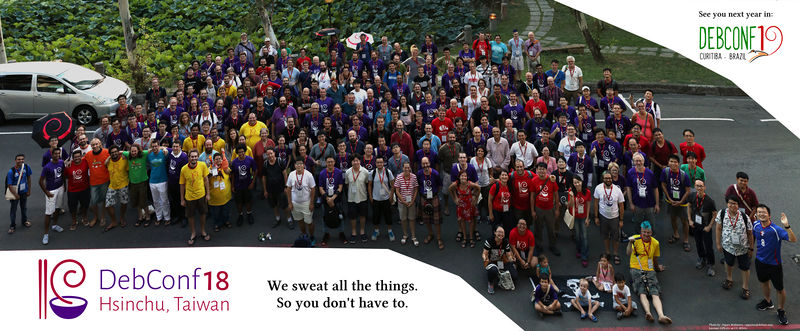
\includegraphics[scale=0.4,bb=0 0 800 331]{image201810/800px-Debconf18_group_photo.jpg}
  \end{center}
  \caption{DebConf18参加者の集合写真}
\end{figure}

セミナー
\begin{itemize}
\item セミナー発表はビデオを公開中 \url{https://debconf18.debconf.org/schedule/}
\item 日本から行った人たちがまとめた参加セミナーの情報
  \begin{itemize}
    \item \url{https://tokyodebian-team.pages.debian.net/2018-08_tokyodebian_debconf18_bof.txt}
  \end{itemize}
\end{itemize}

%%%\includegraphics[scale=0.04]{image201810/IMG_4552.JPG}
% https://wiki.debconf.org/wiki/DebConf18/Photos
%  Aigars Mahinovs (aigarius) - Google Photos
%  https://lh3.googleusercontent.com/h6xIiaSy0Yx9XJOnTpzMlaC2_kymnmKfBDTRuNC9Ori8whzxi4nxvizvrFR_XFEHMrE5z1itgyRG-7FRZPaZDnS8DbiRihCloASeeFBCJjKgvjjCV5pSOkWEDZmfkD_NWrfyESoC_uRYG1NjUd2__FvfNZ3VEQ

\begin{itemize}
\item セミナー発表のタイトルの一部抜粋
  \begin{itemize}
  \item Bits from the DPL
  \item Debian Science BoF
  \item Ignoring Negativity
  \item News from the APT team
  \item Debian Brasil and DebConf19
  \item Debian Diversity Team discussion session
  \item Report from the Debian EFI team about the support of Secure Boot on Debian
  \item Making Debian more user friendly by changing the web start page (www.debian.org)
  \item GDPR in Debian
  \item Debian Go Packaging Team BoF
  \item The Free Software Foundation, Debian, and the free software movement
  \end{itemize}
\end{itemize}


イベント中の生活
\begin{itemize}
  \item Code of Conduct を読み、節度ある生活をする\footnote{\url{https://debconf.org/codeofconduct.shtml}、\url{https://www.debian.org/code_of_conduct}}
  \item ベジタリアン、ハラールの方を考慮した食事を用意
  \item 宿泊は学生寮に滞在可能
  \item wikiを読んで行動する \url{https://wiki.debconf.org/wiki/DebConf18}
  \item お知らせはアナウンスメールを読む \url{https://lists.debian.org/debconf-announce/}
  \item セブンイレブン、ファミリーマートが大学構内にあり便利
  \item 大学内のスポーツ施設を有料で利用可能
\end{itemize}


ハックラボ
\begin{itemize}
\item 今回はNoisy Hacklab、Quiet Hacklabの2部屋を用意
\item インターネット回線、電源を完備
\item コーヒーやビールを飲みながらハックし、議論し、親交を深める
\end{itemize}

%%%\includegraphics[scale=0.025]{image201810/IMG_4534.JPG}
% https://wiki.debconf.org/wiki/DebConf18/Photos
%  Aigars Mahinovs (aigarius) - Google Photos
%  https://lh3.googleusercontent.com/9GbUR4o1QRMyQ9lMZddRM58rEdnk_cXHx9644-3lYyS_hA7TBHFlc1n1gVVr1M0JsjFd6z6mrFxeIOX9HsrbVSW9IeIPSSQcghzYcv52G7GpbrlfCKUhy6zYWOZx70tA_COa4gJG0yhzIbXTiJJ6eitoSLe9pA
%%%\includegraphics[scale=0.025]{image201810/IMG_5065.JPG}
% https://wiki.debconf.org/wiki/DebConf18/Photos
%  Aigars Mahinovs (aigarius) - Google Photos
%  https://lh3.googleusercontent.com/nEnXBYxds7X6H640WGgiAJmPzoHaVST20KM10eOFdVG4BVqo8gjXEMkn4vT40decm2Sl-fbskds-92tos4MBp6-3s8lAG2yUJ2fd-VCtVA60TD9ZXMiXl4zneZ78I8krbFtGxFFrSuevbjqHoWpQMZrEtJR0eQ

DayTrip
\begin{itemize}
\item DebConf中に1日、参加者たちが一緒に出かける企画
\item \url{https://wiki.debconf.org/wiki/DebConf18/DayTrip}
\item 工場見学ツアー、文化施設見学ツアー、お茶会ツアー、台北観光ツアー、自転車でツーリング、川遊び
\end{itemize}

%%%\includegraphics[scale=0.12]{image201810/0801_taipei_1.jpg}
% https://wiki.debconf.org/wiki/DebConf18/Photos
%  Macy- Day trip group photo
%  https://lh3.googleusercontent.com/jnwfbEKoJcPRDn_gSpqxdx8t75FhsMHNKwXUGq75RrNe-7EUDjupBZ4pSqEPqV40yrVp7A1TtDn3ZgWq44HpcZFuVBdLqLAzCgZ8pzXR1QMeqw2F_iglHxs-an-CCp8XRTUdGjTAaE2TJee_8iMFJVkedBY6
%%%\includegraphics[scale=0.16]{image201810/0801_river_4.jpg}
% https://wiki.debconf.org/wiki/DebConf18/Photos
%  Macy- Day trip group photo
%  https://lh3.googleusercontent.com/SqT6u153fNB8ApVeEJe-wyxWeb_Y6XDNcoeYqILGra2uCZ312vhRzLCaq6Wtm_y8xGcAIcCkJ7qA58A6Iu6yog_64p7J49-CYuttE-t_EAYMlvqIvYf2jAlTFobudexvzmdesmb0pb6UY9o80ehzFkLGBQgs


チーズ&ワインパーティ
\begin{itemize}
  \item 自分の国のワインとチーズを持ち寄るホームパーティ
  \item 異文化理解や新たな発見をするための交流の場
  \item \url{https://wiki.debconf.org/wiki/DebConf18/CheeseWineBoF}
\end{itemize}

%%%\includegraphics[scale=0.025]{image201810/IMG_4781.JPG}
% https://wiki.debconf.org/wiki/DebConf18/Photos
%  Aigars Mahinovs (aigarius) - Google Photos
%  https://lh3.googleusercontent.com/j6x2pACKhb2nHKDryGkHUUfkpRYTmqKgJEIF5WctZHlZh9IVL6Qh2A-JGl0Q8VYtxIbUtg7-egzC3zCR7MM6R0O7K60UXVHT36YEF2N_CZo4WEo08KWhkitf-GwJ4kzN9XRjyB99cq7FbI4CLjEpP9lM5MkU6g
%%%\includegraphics[scale=0.025]{image201810/IMG_4790.JPG}
% https://wiki.debconf.org/wiki/DebConf18/Photos
%  Aigars Mahinovs (aigarius) - Google Photos
%  https://lh3.googleusercontent.com/R3lP7_Y_3Kz-yc4TeZSyxC5fQM2t0uUHYcUaXoU_NVFmoudpb7hA6aRveE0F9IiPGxZ4II2WDiC1pzmplroScl2oBLQnB38XT08hBoy2z_VzmLqQmihfxK7g24FqG-Ic10N4JmTSsDXITGdAZaccZrW36NInNA

カンファレンスディナー
\begin{itemize}
  \item 現地の料理を楽しみながら懇親するディナー
  \item スポンサーの方々から挨拶もあります
\end{itemize}

%%%\includegraphics[scale=0.025]{image201810/IMG_5618.JPG}
% https://wiki.debconf.org/wiki/DebConf18/Photos
%  Aigars Mahinovs (aigarius) - Google Photos
%  https://lh3.googleusercontent.com/7Wp_wU_h0mYRZ4_4ZIf1wy7yOyROR8q0JLoijmSzcLq781Fn64aqRaOSCQgJoXCCHw_4aI8vg_-hdy8k-pwTbrJqk0kR2b1sXaxWxJf23WM5zWij6oCHQCLwzziParHa4KJTmxfsmmNIsKpUwqoXFEvGAzkEjQ
%%%\includegraphics[scale=0.025]{image201810/IMG_5641.JPG}
% https://wiki.debconf.org/wiki/DebConf18/Photos
%  Aigars Mahinovs (aigarius) - Google Photos
%  https://lh3.googleusercontent.com/8EKtU1IYlzzwTitBPxoulswKEdISzFY4Wxbqos1zGpbiw-SPR5kQFRWRrCP1G0bZiNciQCfhE52KJ9EwNcCDbnUOTrzNAnr0f1GLPvCnueWNCYpZH65qP9pso4GlFYic-HbWKMVa7YM9cZtQrkyHxPJQk9YBwA


\subsubsection{DebConf19予告}

\begin{itemize}
  \item ブラジル南部のクリチバ市にあるFederal University of Technology(UTFPR)で開催
  \item \url{https://wiki.debian.org/DebConf/19}
\end{itemize}
\begin{figure}[htbp]
  \begin{center}
    
\includegraphics[scale=1.0]{image201810/dc-19-logo.png}
  \end{center}
  \caption{DebConf19ロゴ}
\end{figure}


\subsubsection{Release Schedule}

\begin{itemize}
\item 2018/09/30:  Debian 10 (Buster) Release Schedule
  \begin{itemize}
  \item 2019-01-12 : Transition freeze
  \item 2019-02-12 : Soft freeze
  \item 2019-03-12 : Full freeze
  % https://lists.debian.org/debian-devel-announce/2018/09/msg00004.html
  \end{itemize}
\item Debian 10は2019年中頃のリリースになるのではないかと推測
\end{itemize}


\subsection{日本語によるDebianの情報}

\begin{itemize}
  \item Debian JP Project \\
      \url{https://www.debian.or.jp}
  \item 東京エリアDebian勉強会\\
      \url{https://tokyodebian-team.pages.debian.net/}
  \item 関西Debian勉強会 \\
      \url{https://wiki.debian.org/KansaiDebianMeeting}
  \item Twitter \\
      \url{@debian_jp}
  %\item G+ コミュニティ \\
  %    \url{https://plus.google.com/u/0/communities/106942835439686570073}
  \item  雑誌 Software Design 技術評論社発行
  \begin{itemize}
  \item 「Debian Hot Topics」、GPG関連の記事など(隔月連載)
  \end{itemize}
\end{itemize}

\newpage
\thispagestyle{empty}\mbox{}

\newpage

\begin{center}
本資料のライセンスについて
\end{center}

\begin{fontsize}{6}{6}

本資料はフリー・ソフトウェアです。あなたは、Free Software
Foundation が公表したGNU GENERAL PUBLIC LICENSEの "バージョン2"もしくはそれ以降
が定める条項に従って本プログラムを再頒布または変更することができ
ます。

本プログラムは有用とは思いますが、頒布にあたっては、市場性及び特
定目的適合性についての暗黙の保証を含めて、いかなる保証も行ないま
せん。詳細についてはGNU GENERAL PUBLIC LICENSE をお読みください。

\end{fontsize}

\begin{center}
ソースコードについて
\end{center}

本資料のソースコードは Git を使って\url{git://anonscm.debian.org/tokyodebian/monthly-report.git}
からダウンロードできます。以下に方法を示します。

\begin{commandline}
$ git clone git://anonscm.debian.org/tokyodebian/monthly-report.git
\end{commandline}
%$

\begin{multicols}{2}
 \begin{fontsize}{6}{6}
 \begin{verbatim}
            GNU GENERAL PUBLIC LICENSE
               Version 2, June 1991

 Copyright (C) 1989, 1991 Free Software Foundation, Inc.
    51 Franklin St, Fifth Floor, Boston, MA  02110-1301  USA
 Everyone is permitted to copy and distribute verbatim copies
 of this license document, but changing it is not allowed.

                Preamble

  The licenses for most software are designed to take away your
freedom to share and change it.  By contrast, the GNU General Public
License is intended to guarantee your freedom to share and change free
software--to make sure the software is free for all its users.  This
General Public License applies to most of the Free Software
Foundation's software and to any other program whose authors commit to
using it.  (Some other Free Software Foundation software is covered by
the GNU Library General Public License instead.)  You can apply it to
your programs, too.

  When we speak of free software, we are referring to freedom, not
price.  Our General Public Licenses are designed to make sure that you
have the freedom to distribute copies of free software (and charge for
this service if you wish), that you receive source code or can get it
if you want it, that you can change the software or use pieces of it
in new free programs; and that you know you can do these things.

  To protect your rights, we need to make restrictions that forbid
anyone to deny you these rights or to ask you to surrender the rights.
These restrictions translate to certain responsibilities for you if you
distribute copies of the software, or if you modify it.

  For example, if you distribute copies of such a program, whether
gratis or for a fee, you must give the recipients all the rights that
you have.  You must make sure that they, too, receive or can get the
source code.  And you must show them these terms so they know their
rights.

  We protect your rights with two steps: (1) copyright the software, and
(2) offer you this license which gives you legal permission to copy,
distribute and/or modify the software.

  Also, for each author's protection and ours, we want to make certain
that everyone understands that there is no warranty for this free
software.  If the software is modified by someone else and passed on, we
want its recipients to know that what they have is not the original, so
that any problems introduced by others will not reflect on the original
authors' reputations.

  Finally, any free program is threatened constantly by software
patents.  We wish to avoid the danger that redistributors of a free
program will individually obtain patent licenses, in effect making the
program proprietary.  To prevent this, we have made it clear that any
patent must be licensed for everyone's free use or not licensed at all.

  The precise terms and conditions for copying, distribution and
modification follow.

            GNU GENERAL PUBLIC LICENSE
   TERMS AND CONDITIONS FOR COPYING, DISTRIBUTION AND MODIFICATION

  0. This License applies to any program or other work which contains
a notice placed by the copyright holder saying it may be distributed
under the terms of this General Public License.  The "Program", below,
refers to any such program or work, and a "work based on the Program"
means either the Program or any derivative work under copyright law:
that is to say, a work containing the Program or a portion of it,
either verbatim or with modifications and/or translated into another
language.  (Hereinafter, translation is included without limitation in
the term "modification".)  Each licensee is addressed as "you".

Activities other than copying, distribution and modification are not
covered by this License; they are outside its scope.  The act of
running the Program is not restricted, and the output from the Program
is covered only if its contents constitute a work based on the
Program (independent of having been made by running the Program).
Whether that is true depends on what the Program does.

  1. You may copy and distribute verbatim copies of the Program's
source code as you receive it, in any medium, provided that you
conspicuously and appropriately publish on each copy an appropriate
copyright notice and disclaimer of warranty; keep intact all the
notices that refer to this License and to the absence of any warranty;
and give any other recipients of the Program a copy of this License
along with the Program.

You may charge a fee for the physical act of transferring a copy, and
you may at your option offer warranty protection in exchange for a fee.

  2. You may modify your copy or copies of the Program or any portion
of it, thus forming a work based on the Program, and copy and
distribute such modifications or work under the terms of Section 1
above, provided that you also meet all of these conditions:

    a) You must cause the modified files to carry prominent notices
    stating that you changed the files and the date of any change.

    b) You must cause any work that you distribute or publish, that in
    whole or in part contains or is derived from the Program or any
    part thereof, to be licensed as a whole at no charge to all third
    parties under the terms of this License.

    c) If the modified program normally reads commands interactively
    when run, you must cause it, when started running for such
    interactive use in the most ordinary way, to print or display an
    announcement including an appropriate copyright notice and a
    notice that there is no warranty (or else, saying that you provide
    a warranty) and that users may redistribute the program under
    these conditions, and telling the user how to view a copy of this
    License.  (Exception: if the Program itself is interactive but
    does not normally print such an announcement, your work based on
    the Program is not required to print an announcement.)

These requirements apply to the modified work as a whole.  If
identifiable sections of that work are not derived from the Program,
and can be reasonably considered independent and separate works in
themselves, then this License, and its terms, do not apply to those
sections when you distribute them as separate works.  But when you
distribute the same sections as part of a whole which is a work based
on the Program, the distribution of the whole must be on the terms of
this License, whose permissions for other licensees extend to the
entire whole, and thus to each and every part regardless of who wrote it.

Thus, it is not the intent of this section to claim rights or contest
your rights to work written entirely by you; rather, the intent is to
exercise the right to control the distribution of derivative or
collective works based on the Program.

In addition, mere aggregation of another work not based on the Program
with the Program (or with a work based on the Program) on a volume of
a storage or distribution medium does not bring the other work under
the scope of this License.

  3. You may copy and distribute the Program (or a work based on it,
under Section 2) in object code or executable form under the terms of
Sections 1 and 2 above provided that you also do one of the following:

    a) Accompany it with the complete corresponding machine-readable
    source code, which must be distributed under the terms of Sections
    1 and 2 above on a medium customarily used for software interchange; or,

    b) Accompany it with a written offer, valid for at least three
    years, to give any third party, for a charge no more than your
    cost of physically performing source distribution, a complete
    machine-readable copy of the corresponding source code, to be
    distributed under the terms of Sections 1 and 2 above on a medium
    customarily used for software interchange; or,

    c) Accompany it with the information you received as to the offer
    to distribute corresponding source code.  (This alternative is
    allowed only for noncommercial distribution and only if you
    received the program in object code or executable form with such
    an offer, in accord with Subsection b above.)

The source code for a work means the preferred form of the work for
making modifications to it.  For an executable work, complete source
code means all the source code for all modules it contains, plus any
associated interface definition files, plus the scripts used to
control compilation and installation of the executable.  However, as a
special exception, the source code distributed need not include
anything that is normally distributed (in either source or binary
form) with the major components (compiler, kernel, and so on) of the
operating system on which the executable runs, unless that component
itself accompanies the executable.

If distribution of executable or object code is made by offering
access to copy from a designated place, then offering equivalent
access to copy the source code from the same place counts as
distribution of the source code, even though third parties are not
compelled to copy the source along with the object code.

  4. You may not copy, modify, sublicense, or distribute the Program
except as expressly provided under this License.  Any attempt
otherwise to copy, modify, sublicense or distribute the Program is
void, and will automatically terminate your rights under this License.
However, parties who have received copies, or rights, from you under
this License will not have their licenses terminated so long as such
parties remain in full compliance.

  5. You are not required to accept this License, since you have not
signed it.  However, nothing else grants you permission to modify or
distribute the Program or its derivative works.  These actions are
prohibited by law if you do not accept this License.  Therefore, by
modifying or distributing the Program (or any work based on the
Program), you indicate your acceptance of this License to do so, and
all its terms and conditions for copying, distributing or modifying
the Program or works based on it.

  6. Each time you redistribute the Program (or any work based on the
Program), the recipient automatically receives a license from the
original licensor to copy, distribute or modify the Program subject to
these terms and conditions.  You may not impose any further
restrictions on the recipients' exercise of the rights granted herein.
You are not responsible for enforcing compliance by third parties to
this License.

  7. If, as a consequence of a court judgment or allegation of patent
infringement or for any other reason (not limited to patent issues),
conditions are imposed on you (whether by court order, agreement or
otherwise) that contradict the conditions of this License, they do not
excuse you from the conditions of this License.  If you cannot
distribute so as to satisfy simultaneously your obligations under this
License and any other pertinent obligations, then as a consequence you
may not distribute the Program at all.  For example, if a patent
license would not permit royalty-free redistribution of the Program by
all those who receive copies directly or indirectly through you, then
the only way you could satisfy both it and this License would be to
refrain entirely from distribution of the Program.

If any portion of this section is held invalid or unenforceable under
any particular circumstance, the balance of the section is intended to
apply and the section as a whole is intended to apply in other
circumstances.

It is not the purpose of this section to induce you to infringe any
patents or other property right claims or to contest validity of any
such claims; this section has the sole purpose of protecting the
integrity of the free software distribution system, which is
implemented by public license practices.  Many people have made
generous contributions to the wide range of software distributed
through that system in reliance on consistent application of that
system; it is up to the author/donor to decide if he or she is willing
to distribute software through any other system and a licensee cannot
impose that choice.

This section is intended to make thoroughly clear what is believed to
be a consequence of the rest of this License.

  8. If the distribution and/or use of the Program is restricted in
certain countries either by patents or by copyrighted interfaces, the
original copyright holder who places the Program under this License
may add an explicit geographical distribution limitation excluding
those countries, so that distribution is permitted only in or among
countries not thus excluded.  In such case, this License incorporates
the limitation as if written in the body of this License.

  9. The Free Software Foundation may publish revised and/or new versions
of the General Public License from time to time.  Such new versions will
be similar in spirit to the present version, but may differ in detail to
address new problems or concerns.

Each version is given a distinguishing version number.  If the Program
specifies a version number of this License which applies to it and "any
later version", you have the option of following the terms and conditions
either of that version or of any later version published by the Free
Software Foundation.  If the Program does not specify a version number of
this License, you may choose any version ever published by the Free Software
Foundation.

  10. If you wish to incorporate parts of the Program into other free
programs whose distribution conditions are different, write to the author
to ask for permission.  For software which is copyrighted by the Free
Software Foundation, write to the Free Software Foundation; we sometimes
make exceptions for this.  Our decision will be guided by the two goals
of preserving the free status of all derivatives of our free software and
of promoting the sharing and reuse of software generally.

                NO WARRANTY

  11. BECAUSE THE PROGRAM IS LICENSED FREE OF CHARGE, THERE IS NO WARRANTY
FOR THE PROGRAM, TO THE EXTENT PERMITTED BY APPLICABLE LAW.  EXCEPT WHEN
OTHERWISE STATED IN WRITING THE COPYRIGHT HOLDERS AND/OR OTHER PARTIES
PROVIDE THE PROGRAM "AS IS" WITHOUT WARRANTY OF ANY KIND, EITHER EXPRESSED
OR IMPLIED, INCLUDING, BUT NOT LIMITED TO, THE IMPLIED WARRANTIES OF
MERCHANTABILITY AND FITNESS FOR A PARTICULAR PURPOSE.  THE ENTIRE RISK AS
TO THE QUALITY AND PERFORMANCE OF THE PROGRAM IS WITH YOU.  SHOULD THE
PROGRAM PROVE DEFECTIVE, YOU ASSUME THE COST OF ALL NECESSARY SERVICING,
REPAIR OR CORRECTION.

  12. IN NO EVENT UNLESS REQUIRED BY APPLICABLE LAW OR AGREED TO IN WRITING
WILL ANY COPYRIGHT HOLDER, OR ANY OTHER PARTY WHO MAY MODIFY AND/OR
REDISTRIBUTE THE PROGRAM AS PERMITTED ABOVE, BE LIABLE TO YOU FOR DAMAGES,
INCLUDING ANY GENERAL, SPECIAL, INCIDENTAL OR CONSEQUENTIAL DAMAGES ARISING
OUT OF THE USE OR INABILITY TO USE THE PROGRAM (INCLUDING BUT NOT LIMITED
TO LOSS OF DATA OR DATA BEING RENDERED INACCURATE OR LOSSES SUSTAINED BY
YOU OR THIRD PARTIES OR A FAILURE OF THE PROGRAM TO OPERATE WITH ANY OTHER
PROGRAMS), EVEN IF SUCH HOLDER OR OTHER PARTY HAS BEEN ADVISED OF THE
POSSIBILITY OF SUCH DAMAGES.

             END OF TERMS AND CONDITIONS

        How to Apply These Terms to Your New Programs

  If you develop a new program, and you want it to be of the greatest
possible use to the public, the best way to achieve this is to make it
free software which everyone can redistribute and change under these terms.

  To do so, attach the following notices to the program.  It is safest
to attach them to the start of each source file to most effectively
convey the exclusion of warranty; and each file should have at least
the "copyright" line and a pointer to where the full notice is found.

    <one line to give the program's name and a brief idea of what it does.>
    Copyright (C) <year>  <name of author>

    This program is free software; you can redistribute it and/or modify
    it under the terms of the GNU General Public License as published by
    the Free Software Foundation; either version 2 of the License, or
    (at your option) any later version.

    This program is distributed in the hope that it will be useful,
    but WITHOUT ANY WARRANTY; without even the implied warranty of
    MERCHANTABILITY or FITNESS FOR A PARTICULAR PURPOSE.  See the
    GNU General Public License for more details.

    You should have received a copy of the GNU General Public License
    along with this program; if not, write to the Free Software
    Foundation, Inc., 51 Franklin St, Fifth Floor, Boston, MA  02110-1301 USA


Also add information on how to contact you by electronic and paper mail.

If the program is interactive, make it output a short notice like this
when it starts in an interactive mode:

    Gnomovision version 69, Copyright (C) year  name of author
    Gnomovision comes with ABSOLUTELY NO WARRANTY; for details type `show w'.
    This is free software, and you are welcome to redistribute it
    under certain conditions; type `show c' for details.

The hypothetical commands `show w' and `show c' should show the appropriate
parts of the General Public License.  Of course, the commands you use may
be called something other than `show w' and `show c'; they could even be
mouse-clicks or menu items--whatever suits your program.

You should also get your employer (if you work as a programmer) or your
school, if any, to sign a "copyright disclaimer" for the program, if
necessary.  Here is a sample; alter the names:

  Yoyodyne, Inc., hereby disclaims all copyright interest in the program
  `Gnomovision' (which makes passes at compilers) written by James Hacker.

  <signature of Ty Coon>, 1 April 1989
  Ty Coon, President of Vice

This General Public License does not permit incorporating your program into
proprietary programs.  If your program is a subroutine library, you may
consider it more useful to permit linking proprietary applications with the
library.  If this is what you want to do, use the GNU Library General
Public License instead of this License.
 \end{verbatim}
 \end{fontsize}
\end{multicols}

\begin{center}
Debian オープンユーズロゴ ライセンス
\end{center}

\begin{multicols}{2}
 \begin{fontsize}{6}{6}
 \begin{verbatim}

Copyright (c) 1999 Software in the Public Interest
Permission is hereby granted, free of charge, to any person
obtaining a copy of this software and associated documentation
files (the "Software"), to deal in the Software without restriction,
including without limitation the rights to use, copy, modify, merge,
publish, distribute, sublicense, and/or sell copies of the Software,
and to permit persons to whom the Software is furnished to do so,
subject to the following conditions:

The above copyright notice and this permission notice shall be
included in all copies or substantial portions of the Software.

THE SOFTWARE IS PROVIDED "AS IS", WITHOUT WARRANTY OF ANY
KIND, EXPRESS OR IMPLIED, INCLUDING BUT NOT LIMITED TO THE
WARRANTIES OF MERCHANTABILITY, FITNESS FOR A PARTICULAR PURPOSE AND
NONINFRINGEMENT. IN NO EVENT SHALL THE AUTHORS OR COPYRIGHT HOLDERS
BE LIABLE FOR ANY CLAIM, DAMAGES OR OTHER LIABILITY, WHETHER IN
AN ACTION OF CONTRACT, TORT OR OTHERWISE, ARISING FROM, OUT OF OR
IN CONNECTION WITH THE SOFTWARE OR THE USE OR OTHER DEALINGS IN
THE SOFTWARE.
 \end{verbatim}
 \end{fontsize}
\end{multicols}

% 問題と回答が同じみひらきにならないようにする
%\cleartoevenpage
%-------------------------------------------------------------------------------
%\dancersection{Debian Trivia Quiz 問題回答}{}
%-------------------------------------------------------------------------------

 Debian Trivia Quiz の問題回答です。
 あなたは何問わかりましたか? \\
 %回答はdebianmeetingresume2014-fuyu.jqzというファイルに生成されるので、
 %それを手動でコピペして使う。
 % ここからコピペ
 % FIXME 問題が全部はいったらコピペすること
 %(progn (next-line 1)(insert-file "debianmeetingresume2013-fuyu.jqz") )
%\begin{enumerate}
%\end{enumerate}

% add page to even number
%\newpage
%\cleartoevenpage

\newpage
\thispagestyle{empty}\mbox{}
\newpage

\thispagestyle{empty}
{
\large
\begin{itembox}{\bf 『あんどきゅめんてっど でびあん』について}
本書は、東京および関西周辺で毎月行なわれている『東京エリア Debian 勉強会』および
『関西 Debian 勉強会』で
使用された資料・小ネタ・必殺技などを一冊にまとめたものです。
% FIXME: 範囲を修正すること。
収録範囲は2018/07〜2018/11まで
(関西は対象期間はLT大会やディスカッション主体のため収録無し)
内容は無保証、つっこみなどがあれば勉強会にて。
\end{itembox}
}

\vspace*{16cm}
{\color{dancerlightblue}\rule{\hsize}{1mm}}
\vspace{2mm}

\includegraphics[width=2cm]{image200502/openlogo-nd.eps}
\noindent \Large \bf あんどきゅめんてっど でびあん 2018年冬号\\
\noindent \normalfont 2018年12月30日 \hspace{5mm}  初版第1刷発行\\
\noindent \normalfont 東京エリア Debian 勉強会/関西Debian 勉強会 (編集・印刷・発行)\\
{\color{dancerdarkblue}\rule{\hsize}{1mm}}

\end{document}
